The low Reynolds number is called the creeping, or over-damped
regime. Let us generalize slightly the momentum equation
Eq \ref{eq:NS_usual} to a general volumetric external force $\bff$:
\[
  \rho \frac{d\bfu }{dt} =
  - \nabla p 
  + \mu \nabla^2 \bfu
  + \bff .
\]

We may again cast the equation into reduced form, to get
\[
\rho^* \frac{d\bfu^* }{dt^* } =
-  \nabla^* p^*
+  \frac1{\mathrm{Re}} \nabla^{*2} \bfu^* .
+  \bff^* ,
\]
where $\bff^*= L/(\rho_0 u_0^2) \bff$. 

As $\mathbf{Re}$ is very small, the equation will tend to
\[
0 = - \mathrm{Re} \nabla^* p^* + \nabla^2 \bfu^* + \mathrm{Re} \bff^*
.
\]
All time derivatives are gone from the equation! The only time
variation that is sometimes considered is the case in which $\bff^*$
is a explicit function of time. In this case, the velocity field
adapts instantaneously following the changes in external force. Coming
from previous chapters, devoted to cases where intertial effects are
not negligible, this may come as a surprise --- nevertheless, this is
the correct description of a regime which is important in fields such
as microfluidics and the biological physics of small systems (from
small insects down to large molecules).  Mathematically, the resulting
equation is now linear in the velocity, which makes its treatment
simpler.

An objection could be raised regarding why the pressure gradient and
the external force terms are kept in the equation, despite being
multiplied by the Reynolds number. The answer is that they are not
in fact negligible, as an alternative scaling is employed. This is
discussed in the next section.



\subsection{Kolmogorov flow}

In order to get an idea of the features of the flow (typical speed,
time scale, Reynolds number), we may gain some insight from the
solution from Kolmogorov flow.

This is an exact solution of the momentum equations when there is a
periodic applied force in the $x$ direction that depends on $y$ only
\[
\bff = f_0 \cos\left( \frac{2\pi y}{L} \right) \bfe_x .
\]

In this case, the typical length-scale $L_0$ and velocity $u_0$ are
set by the force. The former is clearly $L_0=L$, but the velocity is
actually part of the solution. It is therefore more convenient to
introduce an alternative way to cast the momentum equation in
non-dimensional form. First, dividing by $f_0$ and going to
dimensionless spacial coordinates:
\begin{equation}
\label{eq:Navier-Stokes_nondim1}
\frac{\rho}{f_0}
\frac{d \bfu}{d t} =
\frac\mu{f_0 L^2} (\nabla^*)^2 \bfu
-\frac 1{f_0 L} \nabla^* p + \bff^*(\bfr^*) .
\end{equation}
The viscous term sets the velocity scale:
\begin{equation}
  \label{eq:reduced_u0}
  u_0 = ( f_0 L^2 ) / \mu .
\end{equation}

On the left hand side of \ref{eq:Navier-Stokes_nondim1}, the total
derivative limits the setting of the time scale: $t_0=L/u_0$. This
means the equation may be written as
\[
\frac{\rho L^3 f_0}{\mu^2}
\frac{d \bfu^*}{d t^*} =
(\nabla^*)^2 \bfu^*
-\nabla^* p^* + \bff^*(\bfr^*) ,
\]
or
\begin{equation}
\label{eq:Navier-Stokes_nondim2}
\mathrm{Re}
\frac{d \bfu^*}{d t^*} =
(\nabla^*)^2 \bfu^*
-\nabla^* p^* + \bff^*(\bfr^*) ,
\end{equation}
where we again find the Reynolds number, given as
\[
  \mathbf{Re}=\frac{\rho L^3 f_0 }{\mu^2}.
\]
This definition looks rather different from the standard one,
$ \mathbf{Re}=\rho L u_0 / \mu$, but upon insertion of
the typical velocity both are seen to coincide.

Notice that the reduced response time is given by the Reynolds number.
This is a sort of ``double-reduced'' time, given by
$t^{**}= t^* / \mathbf{Re}$. A high Reynolds number therefore means a
long reduced time to respond, while a low Reynolds one the response is
very rapid, and the equilibrium solution is reached very fast. Also,
the pressure is reduced as $p^*= p / ( f_0 L ) $.

Let us apply this scaling to the Kolmogorov flow. Assuming that the
resulting velocity, as the driving force, only has an $x$ component
varying on $y$ (as for planar Couette and Poiseuille flows),
\begin{equation}
\label{eq:Kolmo_orig}
  \rho \frac{\partial u_x}{\partial t} =
  \mu \frac{\partial u_x}{\partial y^2} - \nabla p +   f_0 \cos(2\pi y/L)  .
\end{equation}

As in previous flow patterns, we may set the pressure to some constant
value. Therefore, in reduced units (dropping the askterisks for
clarity),
\[
  \mathrm{Re} \frac{\partial u_x}{\partial t} =
  \frac{\partial  u_x}{\partial y^2} u + \cos(2\pi y) .
\]

The solution is easily found:
\[
  u_x = \frac{1}{(2\pi)^2} \left( 1-e^{ - (2\pi)^2 t/Re } \right)
  \cos(2\pi y) .
\]

Putting the scales back in, we find
\[
  u = \frac{ f_0 L^2 }{(2\pi)^2 \mu} \left( 1-e^{- (2\pi)^2 \mu t /
      (\rho L^2) } \right) \cos(2\pi y/L) ,
\]
which indeed can be checked to be the solution to the original
Equation \ref{eq:Kolmo_orig}.


\section{General solution}

In Equation \ref{eq:Navier-Stokes_nondim2}, we may disregard
completely the left hand side if the Reynolds number is very low. This
leads to Stokes' equation:
%, which in dimensionless units is:
\begin{equation}
\label{eq:Stokes}
\mu \nabla^2 \bfu -\nabla p = - \bff(\bfr) .
\end{equation}
As mentioned, this is a \emph{linear} equation for the velocity.  We
may get a general solution to the equation that gives us the velocity
field for any external field, by using Fourier techniques.

In Fourier space all the fields are given as
\begin{align}
\phi(\bfq) &=                    \int d\bfr \, \phi(\bfr) e^{-i\bfq\cdot\bfr}  \\
\phi(\bfr) &= \frac 1{(2\pi)^d}  \int d\bfq \, \phi(\bfq) e^{ i\bfq\cdot\bfr} 
\end{align}

Stokes' equation for Cartesian coordinate $i$ reads
\cite{bray2002theory}
\[
-\mu q^2 \bfu_i(\bfq) - i \bfq_i p(\bfq) = - \bff_i(\bfq) ,
\]
or
\begin{equation}
\label{eq:u_Fourier0}
\bfu_i(\bfq) = \frac 1{\mu q^2}
\left[
  - i \bfq_i p(\bfq) + \bff_i(\bfq) 
\right] .
\end{equation}

Now, the pressure is fixed by incompressibility. The condition
$\nabla\cdot\bfu=0$, reads in Fourier space
\[
  \sum_i\bfq_i\cdot\bfu_i(\bfq) .
\]
Multiplying Equation \ref{eq:u_Fourier0} by $\bfq_i$ and adding up the
$d$ equations:
\[
\sum_i \bfq_i \bfu_i(\bfq) = \frac 1{\mu q^2}
\left[
  - i q^2 p(\bfq) + q_i\bff_i(\bfq) 
\right] =0 .
\]

Therefore,
\[
  - q^2 p(\bfq) = i q_i\bff_i(\bfq)   .
\]
This looks like the Fourier version of a Poisson pressure equation:
\[
  \nabla^2 p = \nabla\cdot \bff .
\]
This is no coincidence, since in \ref{eq:Stokes} we may use the
identity
\(\nabla^2 \bfu = \nabla(\nabla\cdot\bfu -
\nabla\times\nabla\times\bfu \). The first term must be zero for an
incompressible fluid, and applying $\nabla\cdot$ we may get rid of the
first one too (since a rotational field is divergence free). The
Poisson equation results. It is interesting that much the same
equation is found in computational methods that enforce
incompressibility by projection.

The pressure is then
\begin{equation}
\label{eq:p_Fourier0}
p(\bfq) = -i \frac{\sum_i q_i\bff_i(\bfq) }{q^2} .
\end{equation}

With this result we may write Equation \ref{eq:u_Fourier0} as
\begin{equation}
\label{eq:u_sol_Fourier}
\bfu_i(\bfq) = \frac 1{\mu q^2}
\sum_j
\left[ \delta_{ij} - \frac{ \bfq_i  \bfq_j}{q^2} \right]
\bff_j(\bfq) =: \sum_j T_{ij} \bff_j(\bfq),
\end{equation}
%
where the last equation the Oseen tensor is defined:
\[
T_{ij}(\bfq) := \frac 1{\eta q^2} \left[
  \delta_{ij} - \frac{ \bfq_i  \bfq_j}{q^2} 
\right].
\]

In 3D, Equation \ref{eq:p_Fourier0} may be inverted back to real space
to yield \cite{pozrikidis2011introduction}.
\[
p(\bfr) = \frac{\bff\cdot\bfr}{4\pi r^3} .
\]

Oseen's tensor can also be inverted:
\[
T_{ij}(\bfr) :=  \frac 1{8\pi \eta r} 
\left(
  \delta_{ij} + \frac{ \bfr_i  \bfr_j}{r^2}
\right)
\]
But notice Equation \ref{eq:u_sol_Fourier} is a convolution in
real space:
\begin{equation}
\label{eq:u_sol_real}
\bfu_i(\bfr) =  \sum_j \int \,d\bfr' T_{ij}(\bfr'-\bfr) \bff_j(\bfr') .
\end{equation}

In 2D, on the other hand, the Fourier expressions cannot be
inverted. This is the famous ``Stokes paradox'': there are no
solutions to his equation for steady translational motion in 2D (it
also applies to 2D problems in 3D, such as the motion of an infinite
cylinder). In their influential 1975 article
\cite{saffman1975brownian} Saffman and Delbr{\"u}ck discussed several
ways out of this paradox, and found out the most satisfactory way was
to take into account the viscosity of the surrounding liquid,
$ \eta_\mathbf{f}$.

In \cite{lubensky1996hydrodynamics}, Lubensky and Goldstein argued
that this would modify the original Stokes equation as:
\[
\eta_\mathbf{f} \nabla^2 \bfu -\nabla p = - \bff(\bfr) - 2
\eta_\mathbf{f} \int d^2\mathbf{r'} K(\mathbf{r}-\mathbf{r'})
\bfu(\mathbf{r'}) .
\]
(We write $\eta_\mathbf{m}$, m for membrane, for what has been just
$\eta$, since we also have $\eta_\mathbf{f}$.)  The last term reflects
an aditional 2D force on the membrane due to its velocity field,
mediated by the surrounding fluid (the factor of $2$ appears because
there are two fluid regions at each side of the membrane). This
convolution is just a product in Fourier space, and the Fourier
transform of $K$ turns out to be simply $-q$.  The resulting Oseen
tensor is then replaced by:
\begin{equation}
\label{eq:SD}
T_{ij}(\bfq) := \frac 1{\eta_\mathrm{m} (q^2 + q / L_\mathrm{SD})}
\left[ \delta_{ij} - \frac{ \bfq_i \bfq_j}{q^2} \right].
\end{equation}
I.e. the only modification is that the denominator of the original
expression is replaced in this way:
\[
\eta q^2 \rightarrow
\eta_\mathrm{m} (q^2 + q / L_\mathrm{SD}) =
\eta_\mathrm{m} q^2 + 2 \eta_\mathrm{f} q ,
\]
with the Saffman-Delbr{\"u}ck length is given by
\[
L_\mathrm{SD} = \frac{\eta_\mathrm{m} }{ 2 \eta_\mathrm{f} } 
\]
(the 3D and 2D viscosities have different physical dimensions, and
this ratio is indeed a length.)


In Figure \ref{fig:SD} we plot the function $1/(q^2+q)$ in log-log
scale.  At high $q$ (short distances), the denominator approaches
\( \eta_\mathrm{m} q^2 \),
which is the prediction from the standard theory as just described. At
low $q$ (long distances), on the other hand, the denominator
approaches \( 2 \eta_\mathrm{f} q \),
which will cause a convergent real-space Oseen tensor with magnitude
given by the viscosity of the surrounding liquid.

At this stage, I do not know how to implement this correction in real
space, and until I get results I am not convinced it is really that
important.

\begin{figure}
  \centering
  \begin{minipage}{0.45\textwidth}
      \includegraphics[width=\textwidth]{figures/SD}
  \end{minipage}
  \caption{Plot of $1/(q^2+q)$ function
    \label{fig:SD}}
\end{figure}



\subsection{Creeping flow past objects}



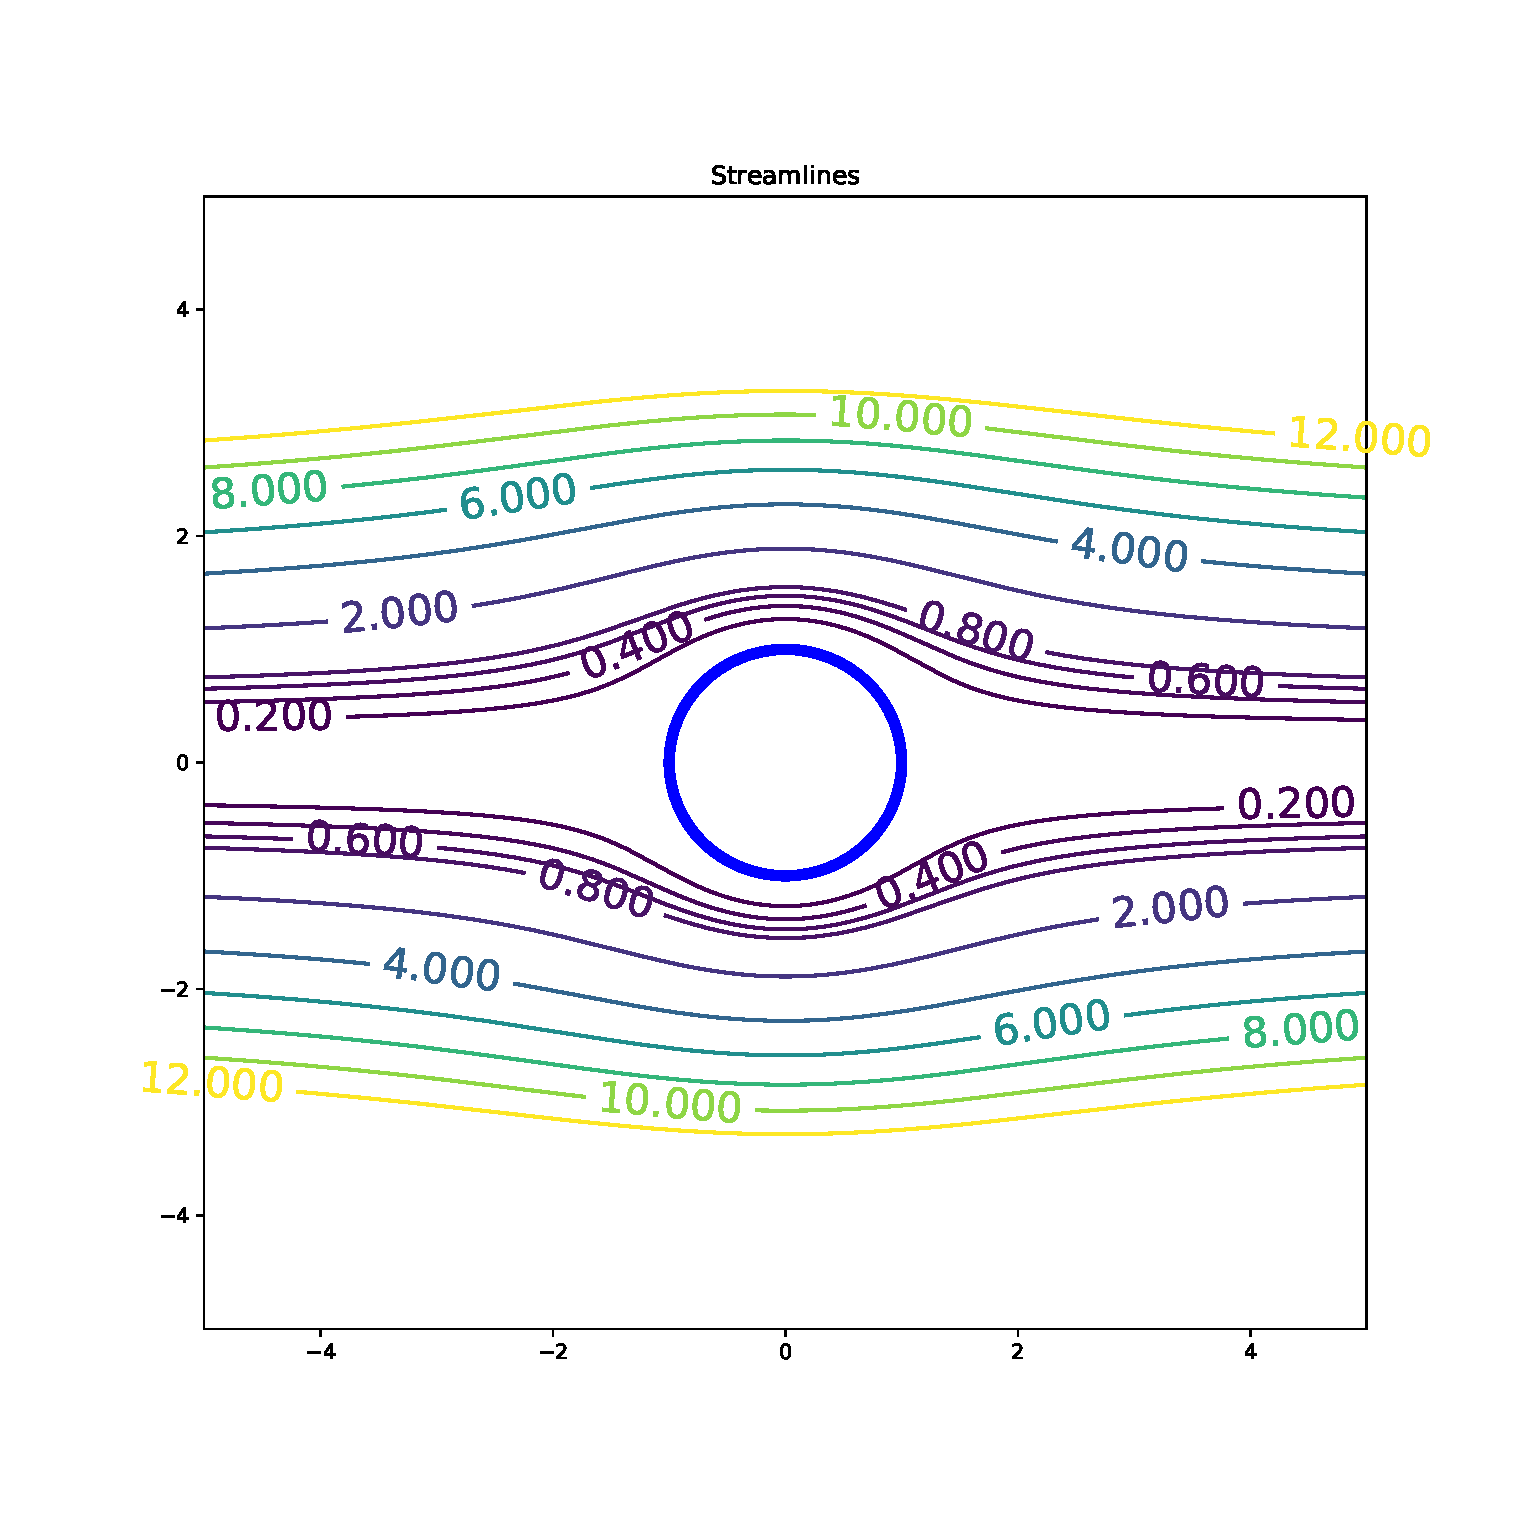
\includegraphics[width=0.8\linewidth]{figures/creeping_flow_past_sphere}

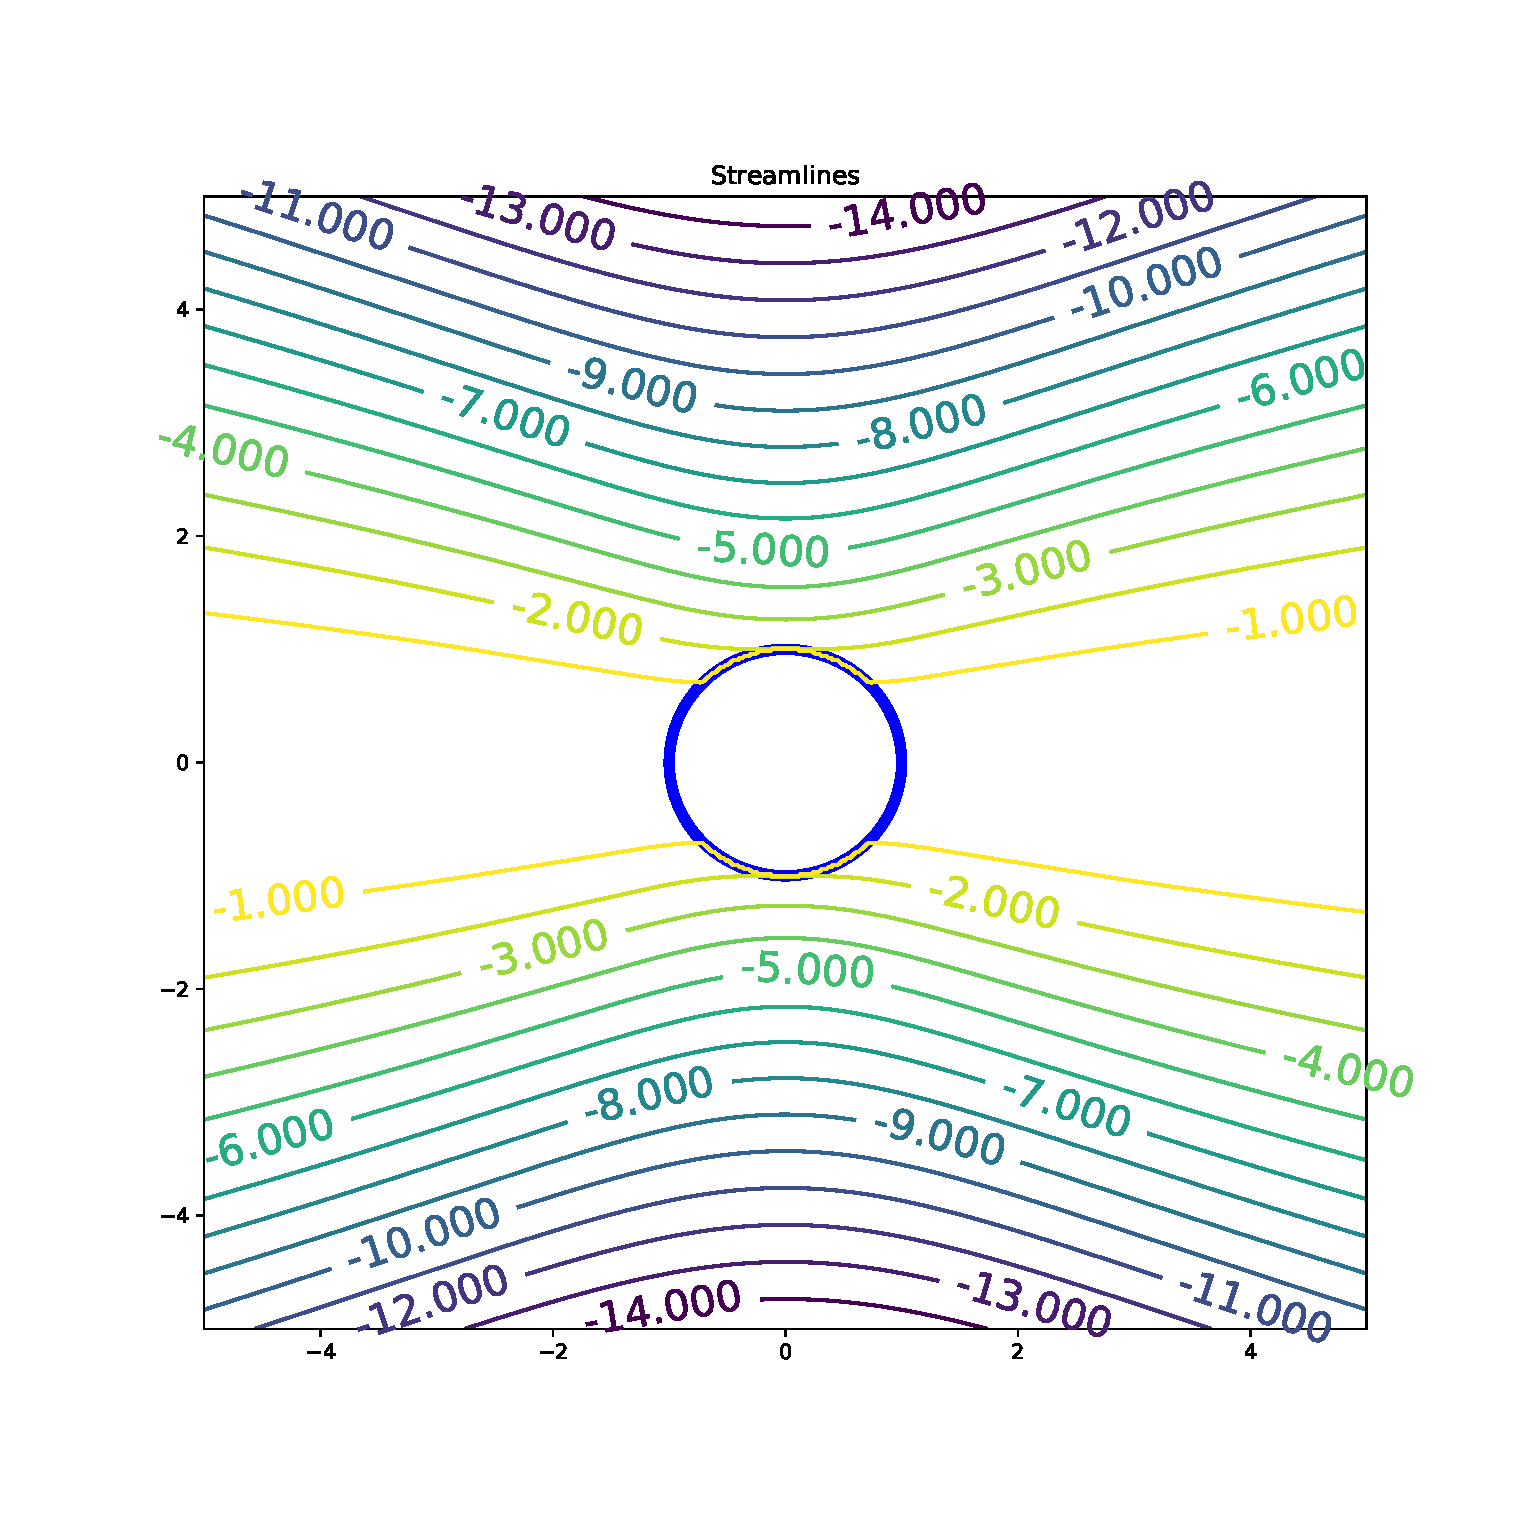
\includegraphics[width=0.8\linewidth]{figures/creeping_flow_past_sphere_moving}
